\chapter{Theoretical background of thermal infrared remote sensing}

\label{Chapter2}

%description
%----------------------------------------------------------------------------------------
This chapter reviews some fundamentals of thermal remote sensing (Section 2.1), as well as a useful approach uses to identify and determine target temperature of sub-pixel resolution (Section 2.2). \\

%----------------------------------------------------------------------------------------
%	SECTION 1
%----------------------------------------------------------------------------------------

\section{Principles of thermal infrared remote sensing}
Thermal remote sensing depends on the fact that any object with a temperature above absolute zero (0 K or -273.15 $^\circ$C) emits electromagnetic (EM) radiation in the infrared range. For example, the Earth we live has an average temperature around 300 K and its peak emittance is near 10 $\mu$m, which falls on thermal infrared domain \parencite {Reference201, Reference202}. The spectral composition and intensity of the emitted radiation are determined by its surface temperature, which is also called kinetic temperature $T_{kin}$,  and the emissivity of the object \parencite{Reference207}. The emissivity $\varepsilon_{\lambda}$, $\varepsilon$ for short, is a ratio of the radiant flux of an object at a certain temperature to the radiant flux of a blackbody at the same temperature (Equation \eqref{eq1}), representing the effectiveness of the object in emitting energy as thermal radiation. The blackbody is an idealized physical object that absorbs and re-emits all incident EM radiations, which means its emissivity is 1 \parencite{Reference206, Reference204}. The emissivity varies as a function of wavelength $\lambda$ and also depends on the surface properiies of the object such as surface roughness or color, but is not temperature-dependent \parencite{Reference203}.\\
\begin{equation}
\label{eq1}
\varepsilon_{\lambda} = \frac{L_{gb, \lambda}(T_{kin})}{L_{bb, \lambda}(T_{kin})}
\end{equation}

\noindent with:\\
\indent $T_{kin}$ = kinetic temperature [K]\\
\indent $L_{gb, \lambda}(T_{kin})$ = radiance of an object with temperature $T_{kin}$ at a certain wavelength [$W m^{-2} sr^{-1} \mu m^{-1}$]\\
\indent $L_{bb, \lambda}(T_{kin})$ = radiance of blackbody with temperature $T_{kin}$ at a certain wavelength [$W m^{-2} sr^{-1} \mu m^{-1}$]\\

% Thus these sensors will produce thermal radiance images which record the equivalent blackbody radiances of the object on the Eearth's surface 
\noindent The satellite remote sensing snesors responsive in the thermal infrared domain are capable to record the EM radiations emited by Earth surface objects \parencite{Reference204}. With the recorded radiation the derivation of the radiant temperature $T_{rad}$ is possible. Radiant temperature $T_{rad}$ is the actual temperature obtained from the measurement of the sensor, representing temperature of a equivalent blackbody \parencite{Reference206}. Notice that the radiant temperature $T_{rad}$ and the kinematic temperature $T_{kin}$ are two different terms and the conversion between them will be introduced later.\\

%-----------------------------------
%	SUBSECTION 1
%-----------------------------------

\subsection{The thermal infrared domain and atmospheric windows}
There is no strict definition of the thermal infrared domain. Usually, the thermal infrared wavelength domain spreads from around 3 to 14 $\mu$m. Within this range, there are two atmospheric windows in the 3 - 5 $\mu$m range and in the 8 - 14 $\mu$m range \parencite{Reference204}. \\

\begin{figure}[!htbp]
  \centering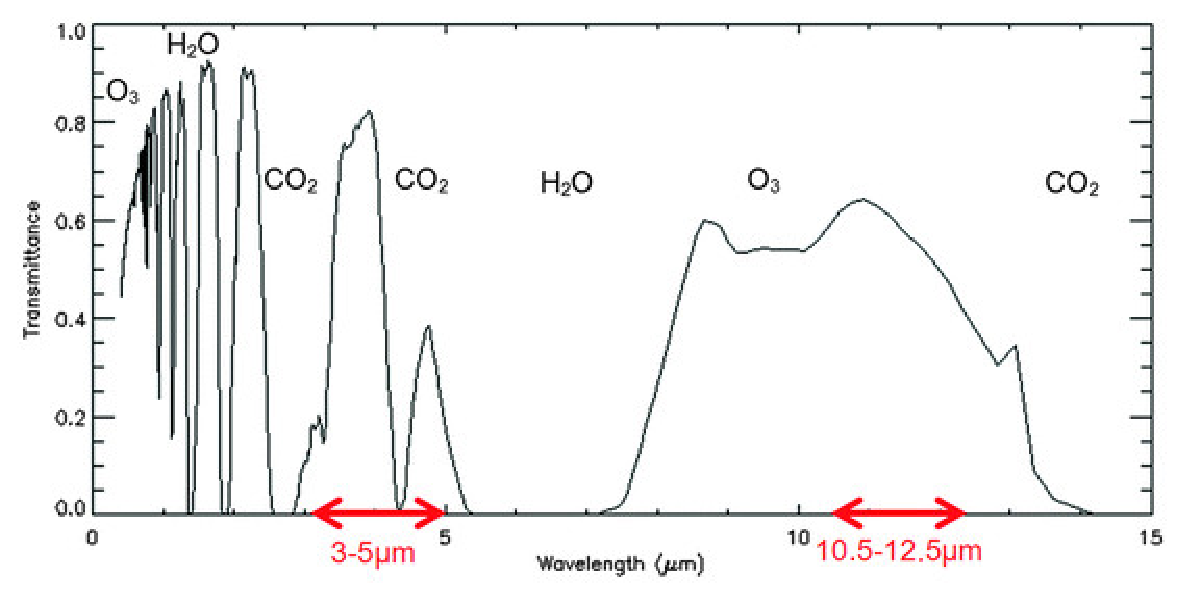
\includegraphics[width=0.8\textwidth]{The_thermal_infrared_wavelength_domain.eps}
  \caption{The thermal infrared wavelength domain \parencite{Reference204}.}
  \label{fig:TIRdomain}
\end{figure}

\noindent The spectral range 8 - 14 $\mu$m, which is called Long-Wavelength InfRared (LWIR), is the thermal imaging region. Within this range, sensors are able to obtain a completely passive image based on the thermal radiation emitted by objects itself and no illumination is required. There is only a absorption of OZone in this region which is neglected by sensors. The spectral range 3 - 5 $\mu$m is called Mid-Wavelength InfraRed (MWIR). Sensors responsive to this spectral range will capture reflected sunlight which contaminates the object-emitted thermal signal. So More attention should be paid when dealing with day-time 3 - 5 $\mu$m MWIR imagery. \\

\noindent For the reason of simplicity, in this thesis, we focus on the night-time TET-1 scene only. \\

%-----------------------------------
%	SUBSECTION 2
%-----------------------------------

\subsection{The Planck's law and Stefan-Boltzmann law}
Planck's blackbody radiation law, Planck's law for short, describes the spectral density of electromagnetic radiation $B_{\lambda}(T_{rad})$ emitted by a blackbody at a given wavelength $\lambda$ as a function of the blackbody's absolute temperature \parencite{Reference208}. Given a certain wavelength $\lambda$, the spectral radiance $B_{\lambda}(T_{rad})$ can be computed from the body's temperature:\\
\begin{equation}
\label{eq2}
B_{\lambda}(T_{rad}) = L_{bb, \lambda}(T_{rad}) = \frac{2hc^2}{\lambda ^5} \frac{1}{e^{\frac{hc}{\lambda k T_{rad}}} - 1}
\end{equation}

\noindent with:\\
\indent $B_{\lambda}(T_{rad})$ = spectral radiance of blackbody with temperature $T_{rad}$ at wavelength $\lambda$\\
\indent $h$ = Planck's constant [$6.626 \cdot 10^{34} J s$]\\
\indent $c$ = speed of light in vacuum [$2.9979246 \cdot 10^8 m s^{-1}$]\\
\indent $\lambda$ = wavelength [$\mu m$]\\
\indent $e$ = Euler's number\\
\indent $k$ = Boltzmann constant [$1.3806 \cdot 10^{-23} J K^{-1}$]\\

\noindent By inverting Equation \eqref{eq2}, the temperature of a blackbody at a certain wavelength $\lambda$ can be calculated.\\
\begin{equation}
\label{eq3}
T_{rad} = B_{\lambda}^{-1}(L_{bb}) = \frac{hc}{k \cdot \lambda \cdot ln(\frac{2hc^2}{L_{bb} \cdot \lambda ^5 \cdot 10^6} + 1)}
\end{equation}

\noindent The Stefan-Boltzmann law describes the power radiated from a blackbody in terms of its temperature \parencite{Reference201, Reference209}.\\
\begin{equation}
\label{eq4}
T_{Radbb} = \sigma T_{kin}^4
\end{equation}

\noindent with:\\
\indent $T_{Radbb}$ = Radiant flux of a blackbody [$W/m^2$]\\
\indent $\sigma$ = Stefan-Boltzmann constant [$5.6697 \cdot 10^{-8} W m^{-2} K^{-4}$]\\

\noindent Through Equation \eqref{eq4} we can obtain the relationship between the radiant temperature $T_{rad}$ and the kinetic temperature $T_{kin}$:\\
\begin{equation}
\label{eq5}
T_{rad} = \sigma ^{\frac{1}{4}} T_{kin}
\end{equation}

\noindent For a blackbody whose emissivity $\varepsilon$ = 1, its radiant temperature $T_{rad}$ equals kinetic temperature $T_{kin}$. For all natural materials with an emissivity $\varepsilon <$ 1, radiant temperature $T_{rad}$ is always lower than kinetic temperature $T_{kin}$.\\

\noindent This is a crucial fact in thermal remote sensing data analysis because it reveals how important the emissivity is: objects with the same radiant temperature $T_{rad}$ measured at sensor might vary significantly in their kinetic temperatures $T_{kin}$ due to the considerable differences among their emissivities.\\

%----------------------------------------------------------------------------------------
%	SECTION 2
%----------------------------------------------------------------------------------------

\section{A dual-channel method for the identification of sub-resolution high temperature sources}
From satellites which contain more than one channel in the thermal infrared spectral region, it is possible to measure surface temperature fields of sub-pixel spatial resolution. Because of the different responses of Planck's function at different wavelength, the radiant temperatures measured in two channels may be expressed in terms of contributions from two temperature fields, each occupying a portion of the pixel \parencite{Reference210, Reference211}.\\

\noindent As mentioned before, The TET-1 satellite's payload including a HSRS with two thermal infrared spectral bands, one MIR band and one TIR band. Assume that the TET-1 scene contains a sub-pixel high-temperature target within one ''hot pixel''. Such a ''mixed pixels'' composes of a target at temperature $T_t$, which we call it effective target temperature, occupying portion $p$, which we call it effective target pixel fraction, of the pixel (where $0 \leqslant p \leqslant 1$) and a background temperature $T_b$ which occupies the remaining portion $(1 - p)$. The measured black body radiance $L_{bb, \lambda}$can be written as:\\
\begin{equation}
\begin{aligned}
\label{eq5}
L_{bb, 1}(T_{rad, 1}) = pL_{bb, 1}(T_t) + (1 - p)L_{bb, 1}(T_b)\\
L_{bb, 2}(T_{rad, 2}) = pL_{bb, 2}(T_t) + (1 - p)L_{bb, 2}(T_b)
\end{aligned}
\end{equation}

\noindent where 1 represents the MIR band and 2 represents the TIR band.\\

\noindent If the background temperature $T_b$ is known from neighbor pixels of the hot pixel, these two equations become two linear equations with two unknowns and can be solved easily. For some applications, there is not reliable estimation of the background temperature $T_b$. Then more complicated method should be applied to solve equations \eqref{eq5}, which goes beyond the scope of this thesis and will no be covered here.\\

\noindent Of course, more than one sub-pixel fire patch might be contained within one hot pixel. Even if only one patch exists, it usually does not have a uniform sub-pixel temperature. This is the reason why we call $T_t$ and $p$ effective, representing an imaginary homogeneous high-temperature event.\\

%----------------------------------------------------------------------------------------
%	SECTION 3
%----------------------------------------------------------------------------------------

%\section{The mitip, an atmospheric correctoin and image processing method}